My Arduino-based project corrects slouching posture. Whenever the wearer slouches, the device buzzes and displays a message on its screen insulting them until they sit upright. The device is operated by simply clipping it onto a shirt or sweater and then powering it on.


\section*{Design and Implementation}

Since the proposal, the tactile button switch to set the wearer's posture to a new default state has been omitted. Additionally, a toggle switch, TFT display, and a breakout board and cable for the display have been added to the list of components.

\subsection*{Parts} % List of all parts and their purposes
The parts for this project include:
	\begin{itemize}
		\item A \href{https://www.adafruit.com/product/2590}{Metro Mini 328} from Adafruit as the Arduino microcontroller.
		\item A \href{https://tinkersphere.com/sensors/315--triple-axis-accelerometer-and-gyro-breakout-mpu-6050.html}{MPU-6050 Accelerometer-Gyroscope} from Tinkersphere as the sensor measuring the positioning of the wearer's torso.
		\item A \href{https://www.adafruit.com/product/1201}{vibrating mini motor disc} from Adafruit to alert the user by buzzing.
		\item A \href{https://www.adafruit.com/product/2305}{DRV2605L Haptic Motor Controller} from Adafruit to control the vibration of the mini motor disc.
		\item A \href{https://www.adafruit.com/product/5206}{ST7789 1.69" 280x240 IPS TFT Display} from Adafruit to display messages.
		\item An \href{https://www.adafruit.com/product/5613}{EYESPI Breakout Board} from Adafruit to extend and organize the wiring needed for the TFT display.
		\item A \href{https://www.adafruit.com/product/5239}{EYESPI Cable} from Adafruit to connect the display and EYESPI breakout board.
		\item A \href{https://www.adafruit.com/product/354}{Lithium Ion battery pack} from Adafruit to power the project.
		\item A \href{https://www.adafruit.com/product/2465}{PowerBoost 1000} from Adafruit to boost the Battery's voltage from 3.7V to 5V.
		\item A toggle slide switch gifted by the course instructor to power off and on the project.
	\end{itemize}


The device is powered by a 3.7V Lithium Ion battery, boosted by the Adafruit PowerBoost 1000 to 5V. The boosted output is then fed into the Arduino and all other components so that they all work at the 5V logic level. The MPU-6050 Accelerometer-Gyroscope and DRV-2605L Haptic Motor Driver are connected to the Arduino using I2C communication, whereas the ST7789 TFT Display is connected to the Arduino using an SPI connection. 

The MPU-6050 serves as the project's sensor, gathering data on the project's orientation, acceleration, and temperature. Using the \href{https://github.com/rfetick/MPU6050\_light/}{MPU\_light} Arduino library by rfetick on GitHub, I was able to fetch these values from the component. In order to sense whether a person is slouching or not, only the orientation values from the MPU-6050 are needed. 
If the pitch angle measured is greater than or equal to 3, then the user is alerted by the buzzing of the vibrating motor disc controlled by the DRV-2605L using the \href{https://github.com/adafruit/Adafruit\_DRV2605\_Library}{Adafruit\_DRV2605} library to trigger the mini motor disc to vibrate. Additionally, the ST7789 TFT display is cleared and displays a new message insulting the wearer. 
Otherwise if the pitch angle is less than 3, the vibrating mini disc does not vibrate and the attached display shows a message complementing the wearer on their good posture. The screen graphics are written to using the \href{ttps://github.com/adafruit/Adafruit-GFX-Library}{Adafruit\_GFX} and \href{https://github.com/adafruit/Adafruit-ST7735-Library }{Adafruit\_ST7789} libraries. 

\begin{figure}[h]
	\centering
	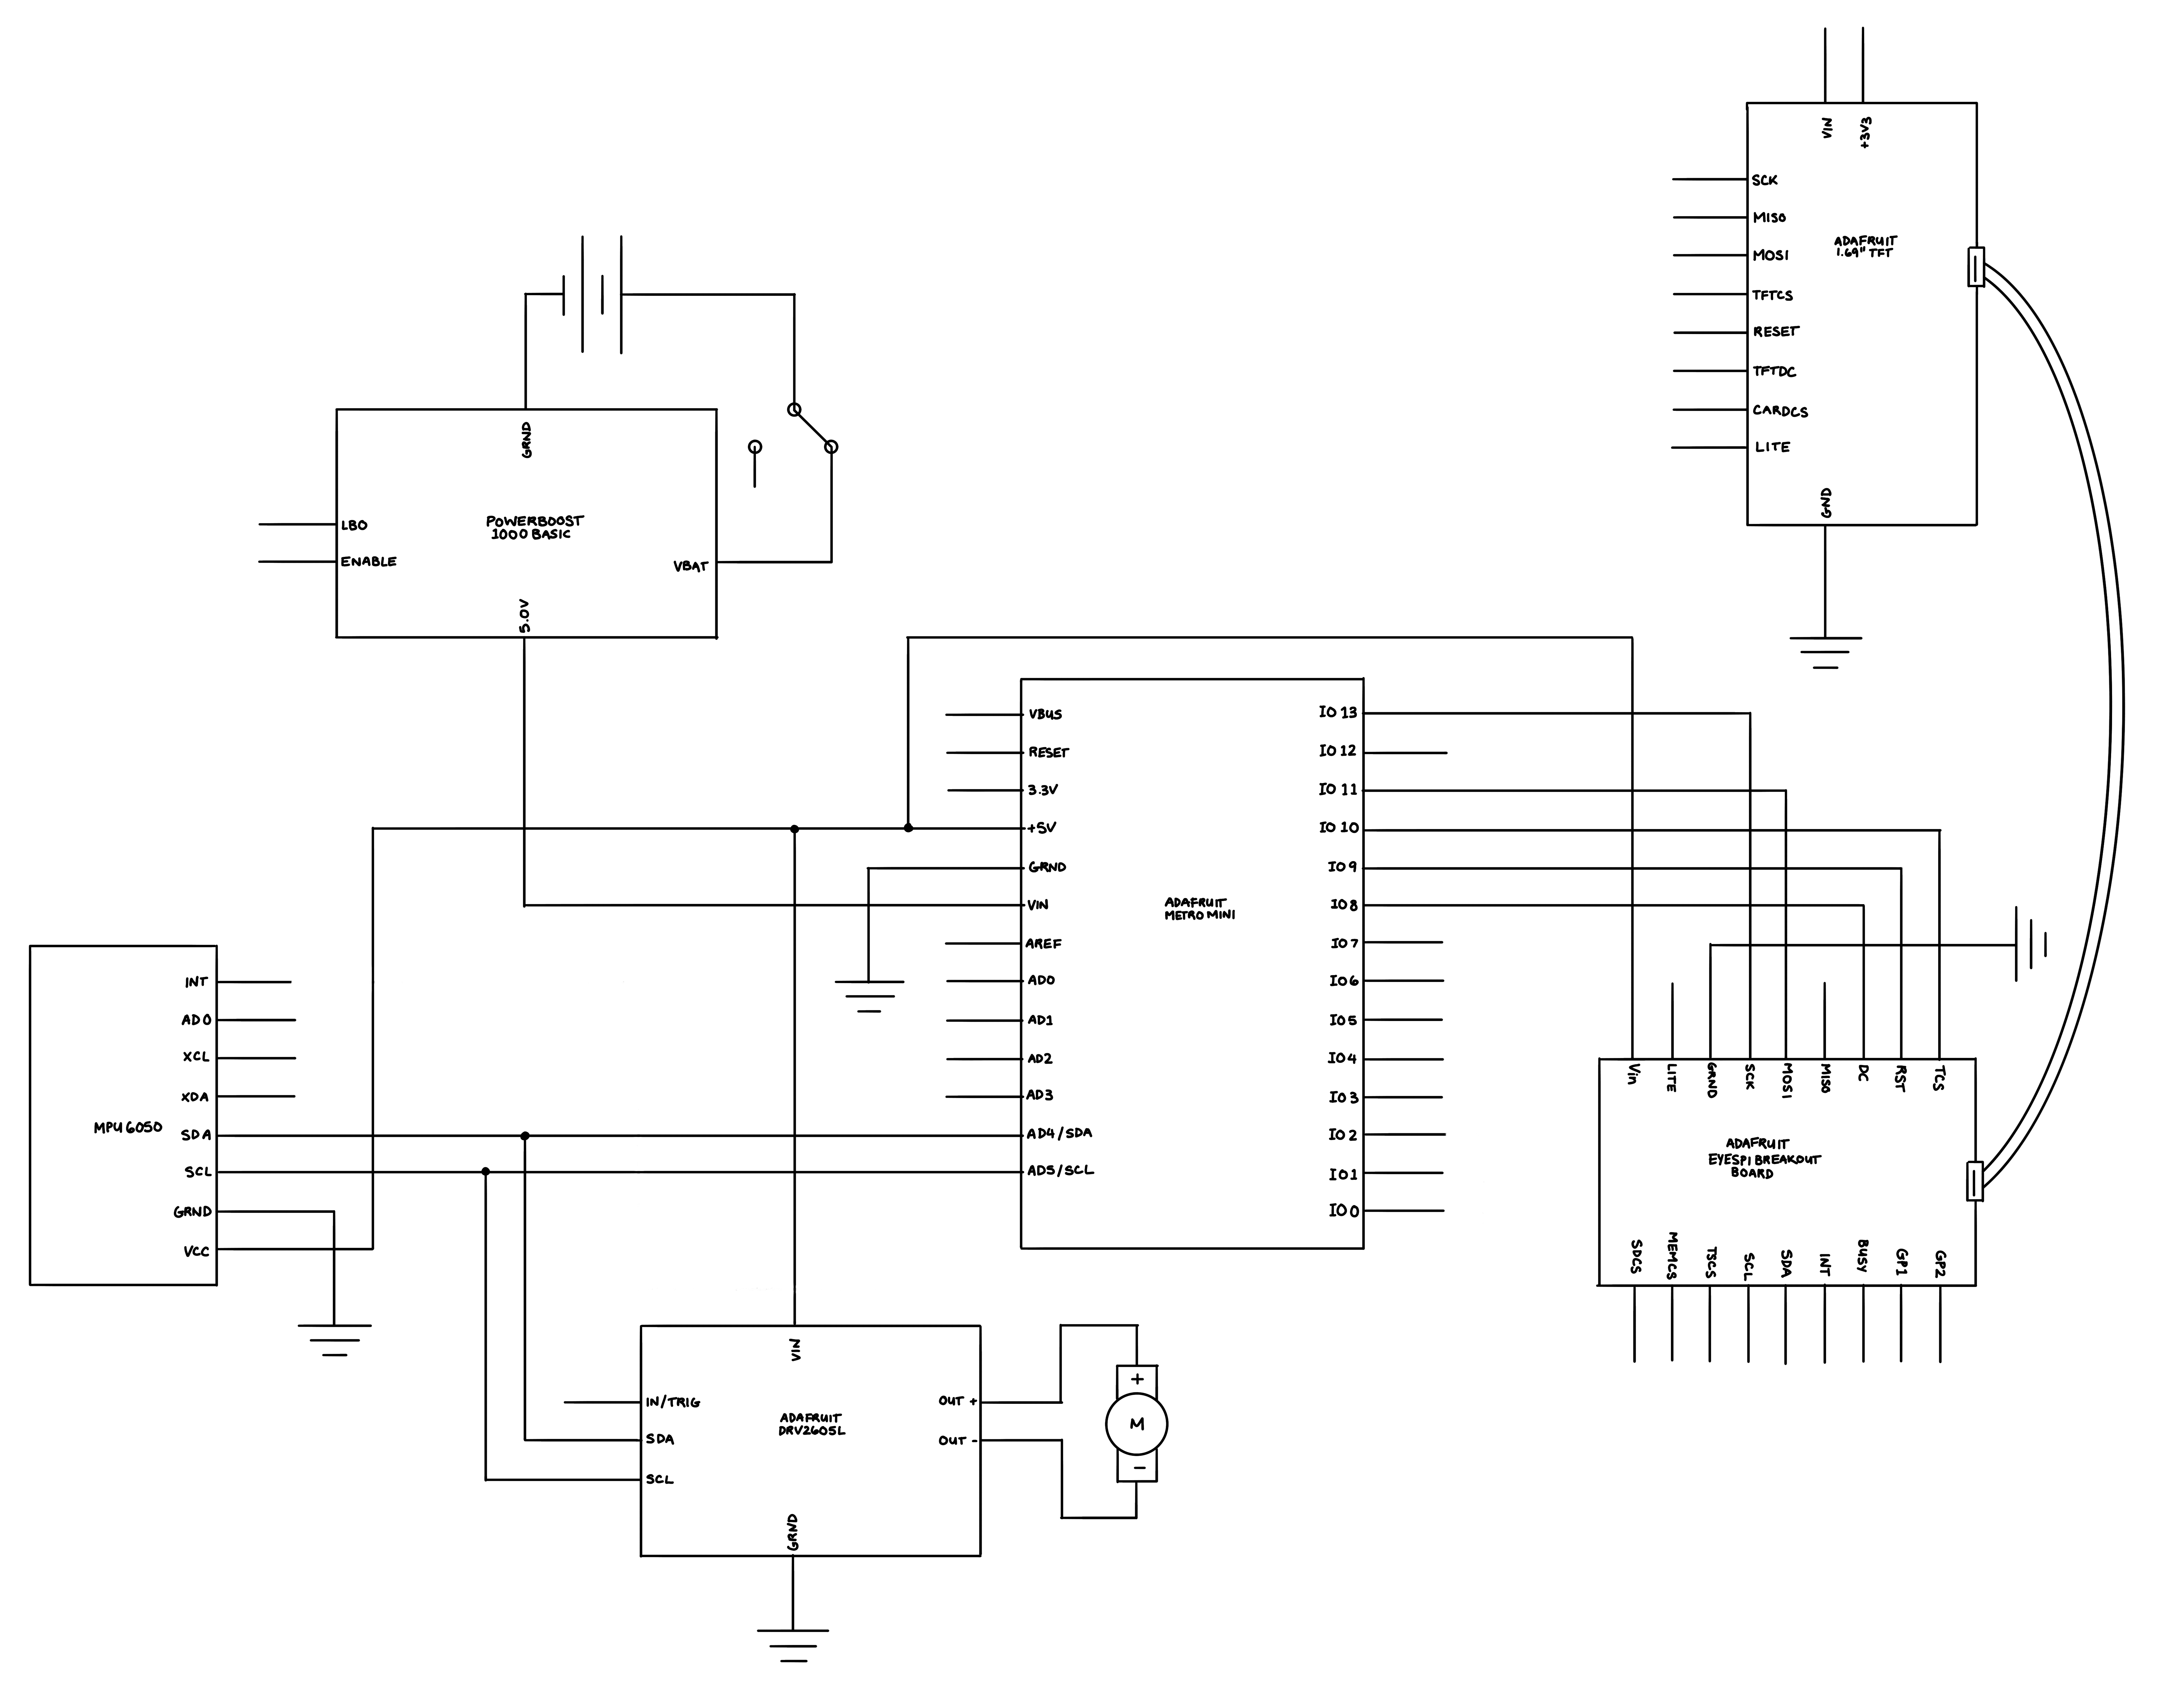
\includegraphics[width=15cm]{schematic.png}
	\caption{Schematic of the Arduino-based posture corrector.}
\end{figure}

When adding the screen to my project, a primary goal of mine was to display a bitmap image of a cat on the display loaded from a micro-SD card. The plan was to have the image varying from a happy cat, to a neutral cat, to an evil cat depending on the pitch value. Though I was successfully able to load the image onto the screen while experimenting with the screen, when incorporated into the sketch written for the project the program was unable to upload onto the Arduino due to the device not having enough RAM memory. Due to this, I opted to only display a text message.

Another goal that I did not achieve with my project was to have it be very small. Though it is still rather small, it is uncomfortable to wear and pulls down on the wearer's shirt more than I would like it to. If I were to remake this project, I would consider using an Arduino LillyPad or Adafruit Flora—rather than the Adafruit Metro Mini—considering they are specifically for wearables. I would also use a smaller battery to reduce the weight of the project.

Lastly, I would have liked to 3D print the case for my project to improve the appearance and polish of the finished project.



\newpage
\section*{References} % References and libraries used
External libraries used:
\begin{itemize}
	\item \href{https://github.com/rfetick/MPU6050\_light/}{MPU6050\_light by rfetick} on GitHub downloaded on 12/18/2022
	\item \href{https://github.com/adafruit/Adafruit\_DRV2605\_Library}{Adafruit\_DRV2605 by AdaFruit Industries} downloaded on 11/16/2022
	\item \href{https://github.com/adafruit/Adafruit-GFX-Library}{Adafruit\_GFX by AdaFruit Industries} downloaded on 11/28/2022
	\item \href{https://github.com/adafruit/Adafruit-ST7735-Library }{Adafruit\_ST7789 by AdaFruit Industries} downloaded on 11/28/2022 
\end{itemize}

{ \parindent0pt
Some code adapted from:
\begin{itemize}
	\item GetAngle example sketch from the MPU6050\_light library
	\item graphicstest example sketch from the Adafruit\_ST7789 library
\end{itemize}
}
